\documentclass[10pt]{article}

\usepackage{listings}

\usepackage{graphicx}
\usepackage{natbib}

%% THE USEPACKAGES NECESSARY FOR THIS EXAMPLE
%% NOTE THAT genetics_manu_style MUST BE CALLED AFTER mychicago
% \usepackage{graphicx}
 \usepackage{endfloat}
 \usepackage{amsfonts}
 \usepackage{subfigure}
% \usepackage{genetics_manu_style}
 \usepackage{siunitx}
 \sisetup{output-exponent-marker=\ensuremath{\mathrm{E}}}
 
\newcommand{\beginsupplement}{%
        \setcounter{table}{0}
        \renewcommand{\thetable}{S\arabic{table}}%
        \setcounter{figure}{0}
        \renewcommand{\thefigure}{S\arabic{figure}}%
     }

% % Add hyperlinks
% %\usepackage{hyperref}

% % amsmath package, useful for mathematical formulas
 \usepackage{amsmath}
% % amssymb package, useful for mathematical symbols
 \usepackage{amssymb}

% % graphicx package, useful for including eps and pdf graphics
% % include graphics with the command \includegraphics
% \usepackage{graphicx}

% % cite package, to clean up citations in the main text. Do not remove.
% %\usepackage{cite}
 \usepackage{natbib}
 \bibpunct{(}{)}{;}{author-year}{}{,} 

\usepackage[dvipsnames]{xcolor}

% % Use doublespacing - comment out for single spacing
 \usepackage{setspace}

% % For splitting/combining figures.
 \usepackage{subfigure}

% % Use doublespacing - comment out for single spacing
 \usepackage{setspace} 
% %\doublespacing

% % Split table cells
% %\usepackage{slashbox}

% % Table with curly braces
 \usepackage{multirow,bigdelim}

% % Underline 
 \usepackage[normalem]{ulem}


\newcommand{\St}{\mathcal{S}}
\newcommand{\It}{\mathcal{I}}
\newcommand{\Rt}{\mathcal{R}}
\newcommand{\traj}{\mathcal{V}}

\newcommand{\tree}{\mathcal{T}}

\newcommand{\comment}[1]{{\color{red} (#1)}}

\newcommand{\stochCoalSIR}{stochastic coalescent SIR}
\newcommand{\deterCoalSIR}{deterministic coalescent SIR}

\newcommand{\StochCoalSIR}{Stoch. Coal. SIR}
\newcommand{\DeterCoalSIR}{Deter. Coal. SIR}


\newcommand{\stochSIR}{stochastic SIR}
\newcommand{\StochSIR}{Stochastic SIR}
\newcommand{\BDSIR}{BDSIR}

\title{Supporting material for ``Inferring epidemiological dynamics with Bayesian coalescent inference:  The merits of deterministic and stochastic models''}
\date{}

%% BEGIN DOC
\begin{document}

\maketitle{}

% \begin{center}
% \LARGE{Epidemic Parameter Inference with Coalescent SIR} \\
% \Large{Supplementary Material}
% \end{center}

\section{Sampling from the prior}

In order to assess the correctness of our implementation of the
deterministic coalescent SIR and stochastic coalescent SIR models, for
each model we used the MCMC algorithm to sample trees from the
corresponding distribution $f(\tree|\eta)$, and compared these samples
with coalescent trees simulated directly under the model.

The chosen $\eta$ included $\beta=7.5\times 10^{-4}$, $\gamma=0.3$,
$S_0=999$ and $z_0=30$. The comparisons were performed for trees
generated from 20 leaves, sampled at integer times 0 through 19,
inclusive.

For the deterministic coalescent SIR model, the direct simulation
involved numerically solving the Eqs.~(1)--(3) in the main text for
$t\in[0,30]$ and using this solution in combination with Eq.~(10)
in the main text to determine the instantaneous coalescent rate
$\lambda(\tau)$. This rate was used to simulate each of the coalescent
trees in the usual fashion for heterochronous leaf times.  In the case
that the MRCA was not reached before the origin time of the epidemic,
the tree was discarded and the simulation repeated.

The direct simulation proceeded in a similar way for the stochastic
coalescent SIR model, the major difference being that the
stochasticity of this model required each coalescent tree to be
simulated under a distinct realization of the stochastic trajectory.

Comparisons between the direct simulation and MCMC results are shown
in Figures \ref{fig:detCoalValidation} and
\ref{fig:stochCoalValidation} for three different summary
statistics and show very close agreement.

\vspace{3 mm}

\section{Validation through simulated data analysis}
As part of the validation of our implementation of the two coalescent SIR models, trees were 
simulated by their own methods (using stochastically- and deterministically-generated SIR trajectories, 
as discussed in the Methods section of the main paper), and relevant epidemiological parameters were inferred using the 
stochastic and deterministic coalescent SIR models.  Tables 1 and 2 show the results of these analyses, 
indicative of correct implementations. 

Analyses for varying $R_0$ (and necessarily, slightly varied other parameters, such as the birth rate $\beta$) are provided 
in Tables S3 and S4.  Results from tests of the influence of broader priors (with larger standard deviations in log space) are shown in Table S4.  
It appears that allowance of broader priors reduces 95\% HPD coverage in some cases (e.g., for parameter $R_0$) when using the \deterCoalSIR{} inference model, as they increase error and bias.

Finally, it was noticed that even for the higher true parameter values of $R_{0}=2.50$ and $S_{0}=999$, under which \deterCoalSIR{} is expected to 
perform relatively well, there was an inability to accurately estimate the origin parameter $z_0$.  Figure S3 provides some insight into 
this conundrum by examining the trajectories used for tree simulation and subsequent analysis. 

\subsection{H1N1 data selection}

Initially, the H1N1 dataset contained 45 sequences.  The ages of the inferred trees (Figure S4) using the original 45 sequences 
extended more than 1.5 years into the past for each of the SIR models, which is contrary to what we expect for a single, current strain of seasonal influenza.  
Three taxa (labelled 32197, 31893, and 31988) were hypothesized to belong to a unique strain, e.g., an additional seeding from outside the 
Canterbury region or a low-lying previous strain.  Removing these three taxa caused the inferred trees to behave as expected, i.e., tree heights and 
epidemic origin $z_0$ less than a year old.  It also raised the estimated $R_0$ values for all three SIR models (initially 1.24, 1.10, and 1.55 for \stochCoalSIR{}, 
\deterCoalSIR{}, and \BDSIR{}, respectively), as well as those for $\gamma$ (initially 8.74, 12.65, and 11.33 for \stochCoalSIR{}, 
\deterCoalSIR{}, and \BDSIR{}, respectively).  

It will be interesting to further investigate the interplay between influenza strains and its contribution to the overall dynamics.  
For the closed SIR models discussed in this manuscript, however, this additional complexity leads to increased chance of model misspecification and misleading results.  
Therefore, we focused our attention on the analyses using 42 sequences.


\subsection{HIV-1 data analysis}

The original HIV-1 dataset \citep{Hue:2005} was agglomerated from both acute and chronic 
infections sampled in the United Kingdom (UK) and constitutes six phylogenetic clusters, 
from which the five used here (Clusters 1-4 and 6) were drawn.  These particular clusters, with the omission of Cluster 5, were chosen simply 
for the purpose of direct comparison with \cite{Kuhnert:2014}.  Our extension to the 
models allowed us to imprint respective tip dates on the sequence data, sampled from 1999 
to 2003, for inclusion in the likelihood computation. 

For the selected five clusters, the nucleotide alignments 
contained 41, 62, 29, 26, and 35 sequences, respectively, each with 952 sites.  The substitution scheme 
chosen for phylogenetic analysis was the symmetric and independent general time reversible 
model (GTR), with gamma distributed rate variation and explicit proportion of invariable sites (GTR+G+I).  Following \cite{Hue:2005}, the substitution rate 
was set to $\num{2.55}$\mbox{\sc{e}-4} substitutions per site per year.  All other parameters were estimated conjointly, 
and the Bayesian prior distributions are presented in Table 4:  Bayesian prior distributions.

The pathophysiology of HIV is multifarious, and the patterns of its advancement within an 
infected host change throughout time.  In addition to increased complexity potentially caused by recombination events, the transition between HIV's acute and 
chronic phases alters the host's infectivity \citep{Guss:1994}.  The SIR compartmental 
model used for this particular phylodynamic analysis on the UK cluster data does not 
allow for independent infection rates for the acute and chronic phases (but see \cite{VolzFrost:2012} and \cite{Volz:2013}).   However, 
in this study we did not attempt to estimate the infection rate $\beta$ and thus did not 
expect such a difference to significantly impact the estimation of the parameters of 
interest:  the basic reproductive number $R_0$, removal rate $\gamma$, size of the initial susceptible population 
$S_{0}$, and origin of the outbreak $z_{0}$.  


\subsubsection{HIV-1 inference results}  

In regard to parameter inference from the serially-sampled HIV-1 sequence data, the \stochCoalSIR{}, \deterCoalSIR{}, and \BDSIR{} methods were most alike in 
light of the $R_{0}$ results.  The medians and HPD intervals for all clusters pertaining to this parameter,
(especially Clusters 1, 2, 3, and 6), were very close, and those of Cluster 4 were still congruent across the three analyses (Figure S5).  

The coalescent SIR models and \BDSIR{} disagreed with respect to the age of the most recent common ancestor and the origin $z_0$ (Figure S6).  The coalescent SIR models also exhibited much larger 95\% HPD intervals for $z_0$ in each of the clusters; 
while \BDSIR{} encompassed an average of 16 years, the \stochCoalSIR{} and \deterCoalSIR{} models had averages of 49 and 37 years, respectively.   
Furthermore, the estimated age of the common ancestor of the tree was older under the coalescent SIR
models than the estimates reported by either \BDSIR{} or the original data analysis \citep{Hue:2005} for each cluster.  This was also true for the time of origin for the epidemic, 
although for certain clusters the differences between the coalescent estimates of the origin $z_0$ and the birth-death estimates were much greater than others (e.g., Cluster 3).   

The estimates of removal rate $\gamma$ 
from Clusters 1 and 6 were very similar across the three methods (Figure S7).  However, both coalescent SIR
models estimated considerably higher $\gamma$ values for Clusters 2-4 than BDSIR.  This is reflective of the simulation study results, where the two coalescent models 
did not perform as well as \BDSIR{} for the removal parameter.

Median estimates for the initial susceptible population $S_0$ were quite similar in all methods for Clusters 1-4, although \BDSIR{} displayed much wider HPD intervals than \stochCoalSIR{} and \deterCoalSIR{} (Figure S8).
In Cluster 6, the coalescent SIR models showed the smallest HPD intervals for their individual analyses on each cluster, while the opposite was true for \BDSIR{}.  
There was also a disparity between the median estimates for the two coalescent approaches and that of \BDSIR{} for Cluster 6. 
To this effect, it should be noted that the 
number of infections accrued throughout the duration of the epidemic was reported as $N_{e}=1,350$ by Hu{\'e} \textit{et al.}  %so N_e is not equal to S_0 though.... thus I do not understand the comparison to S_0 estimates. I assume that N_e in Hue is the inverse of coalescnet rate. thus,  N_e(\tau) = \It(\tau)/(2{\beta}\St(\tau)).
This casts some suspicion on the low susceptible population estimates obtained by the \stochCoalSIR{} and 
\deterCoalSIR{} methods (median estimates of $S_{0}=727$ and $S_{0}=693$, respectively), since they appear lower than the estimated number of infected individuals from the original study.

There is disagreement in the literature in regard to the modelling of HIV-1 evolutionary dynamics under stochastic or deterministic processes \citep{Nijhuis:1998,Rouzine:1999,Achaz:2004,Shriner:2004}.
The predicament dwells in the observation that the actual effective population size $N_e$ for HIV-1 is often smaller 
than the total population size \citep{Kouyos:2006}.
While most of this debate has focused on within-host population dynamics, many of the arguments hold when considering the broader epidemic dynamics of host-to-host transmission.
As previously mentioned, the  appropriateness of these descriptions is hinged on the magnitude of the infected population, precisely, the effective infected population size. Consequently, even when the total infected population is quite large there may yet be significant stochastic effects in play.

Finally, as mentioned in the main article, the existence of two distinct infectious stages and the possibility of large effects due to recombination are reasons for any discrepancy produced by these SIR inference models.

\subsubsection{Example XML} 

Below is an example XML for simulating 100 trees and trajectories in MASTER \citep{Vaughan:MASTER}.  This example is for $R_0=2.4975$ and $S_0=999$.  
The simulation ends when the infected $I$ population returns to zero, i.e., when the last infected individual is removed.

\lstset{
  basicstyle=\ttfamily,
  columns=fullflexible,
  showstringspaces=false,
  commentstyle=\color{gray}\upshape
}

\lstdefinelanguage{XML}
{
  morestring=[b]",
  morestring=[s]{>}{<},
  morecomment=[s]{<?}{?>},
  stringstyle=\color{black},
  identifierstyle=\color{darkblue},
  keywordstyle=\color{cyan},
  morekeywords={xmlns,version,type}% list your attributes here
}

\footnotesize{
\begin{lstlisting}

<beast version=`2.0' 
namespace=`master.beast:beast.core.parameter:beast.evolution.tree.TreeHeightLogger'>

    <run spec=`InheritanceEnsemble'
	 nTraj=`100'
	 samplePopulationSizes=`true'
	 verbosity=`1'>

        <model spec=`InheritanceModel' id=`model'>
            <population spec=`Population' id=`S' populationName=`S'/>
            <population spec=`Population' id=`I' populationName=`I'/>
            <population spec=`Population' id=`R' populationName=`R'/>
            <population spec=`Population' id=`Rh' populationName=`Rh'/>
            
            <!-- infection reaction -->
            <reaction spec=`InheritanceReaction' reactionName=`Infection' rate=`0.00075'>
                S + I -> 2I
            </reaction>
            
            <!-- recovery reaction -->
            <reaction spec=`InheritanceReaction' reactionName=`Recovery' rate=`0.25'>
                I -> R
            </reaction>
            
            <!-- sampling reaction -->
            <reaction spec=`InheritanceReaction' reactionName=`Sampling' rate=`0.05'>
                I -> Rh
            </reaction>
        </model>

        <initialState spec=`InitState'>
            <populationSize spec=`PopulationSize' population=`@S' size=`999'/>
            <lineageSeed spec=`Individual' population=`@I'/>
        </initialState>

	<populationEndCondition spec=`PopulationEndCondition'
				population=`@I'
				threshold=`0'
				exceedCondition=`false'/>

	<inheritancePostProcessor spec=`LineageFilter'
				  reactionName=`Sampling'
				  discard=`false'/>
		
        <output spec=`NewickOutput' fileName=`SIR.newick'/>
        <output spec=`NexusOutput' fileName=`SIR.nexus'/>
        <output spec=`JsonOutput' fileName=`SIR.json'/>

    </run>
</beast>
\end{lstlisting}}

\beginsupplement
\begin{figure}
  \vspace{-3cm}

    \begin{center}
      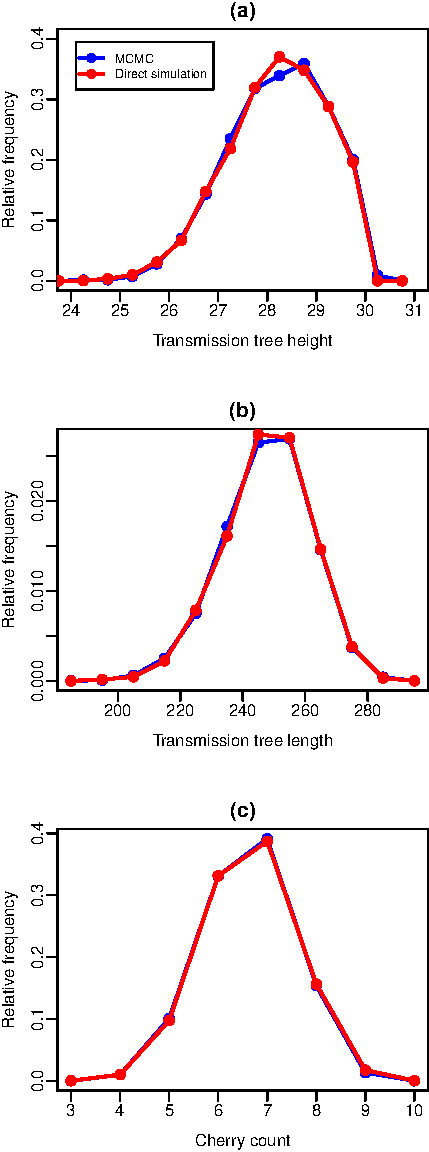
\includegraphics[width=0.6\textwidth]{detCoalFigure-crop.pdf}
    \end{center}
    \caption{Comparison between distributions of summary statistics of
      trees sampled using MCMC employing our implementation of the
      \emph{deterministic coalescent SIR model} likelihood and those
      calculated, and those of trees sampled using direct
      simulation. Summary statistics shown are (a) the age of the MRCA
      of the transmission tree, (b) the sum of all edge lengths in the
      tree, and (c) the total number of two-leaf clades in the tree.}
    \label{fig:detCoalValidation}
\end{figure}

\begin{figure}
  \vspace{-3cm}

    \begin{center}
      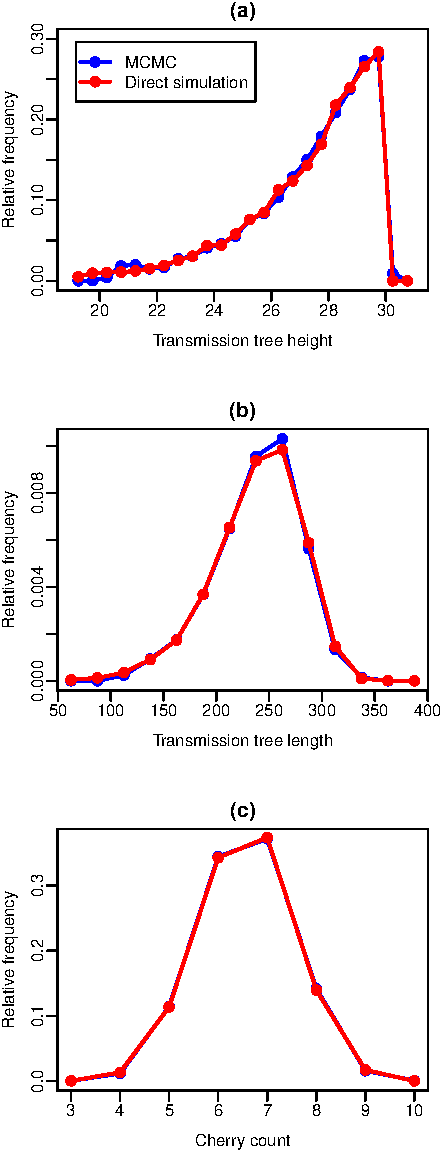
\includegraphics[width=0.6\textwidth]{stochCoalFigure-crop.pdf}
    \end{center}
    \caption{Comparison between distributions of summary statistics of
      trees sampled using MCMC employing our implementation of the
      \emph{stochastic coalescent SIR model} likelihood and those
      calculated, and those of trees sampled using direct
      simulation. Summary statistics shown are (a) the age of the MRCA
      of the transmission tree, (b) the sum of all edge lengths in the
      tree, and (c) the total number of two-leaf clades in the tree.}
    \label{fig:stochCoalValidation}
\end{figure}

\begin{figure}
  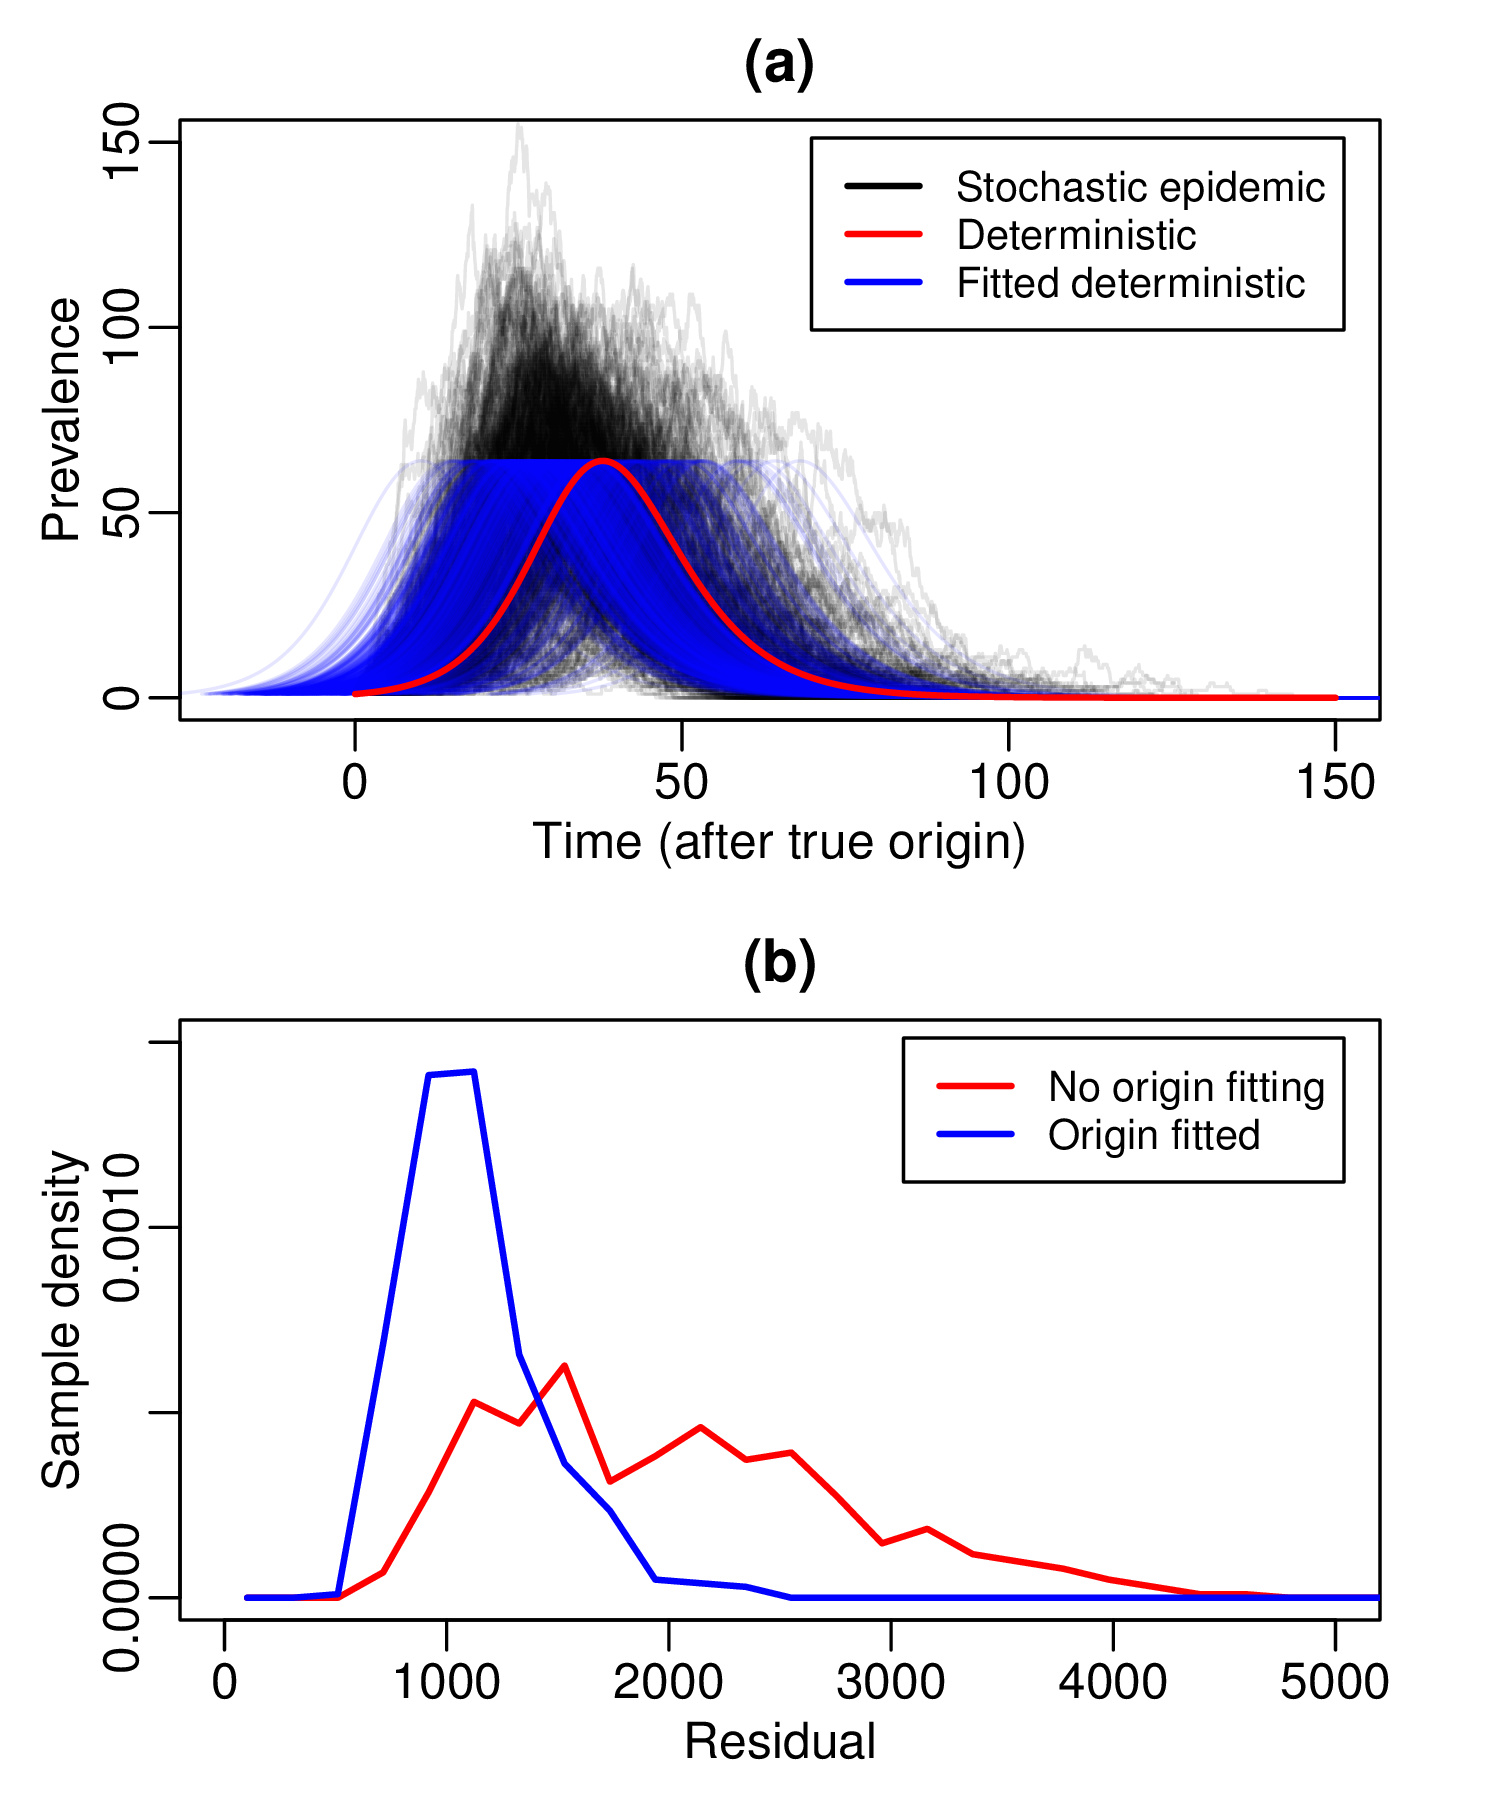
\includegraphics[width=\textwidth]{originFitFigure.jpg}
  \caption{(a) True stochastic SIR trajectories simulated jointly alongside phylogenies, with 
  the corresponding trajectories used by \deterCoalSIR{}.  Adjusting \deterCoalSIR{} 
  to fit the underlying stochastic trajectories causes major shifts to the origin $z_0$.  
  (b) Deterministic residuals with $z_0$ either fitted or not.}
  \label{fig:originFit}
\end{figure}
%
%
\begin{figure}[ht]
    \centering
{%
    	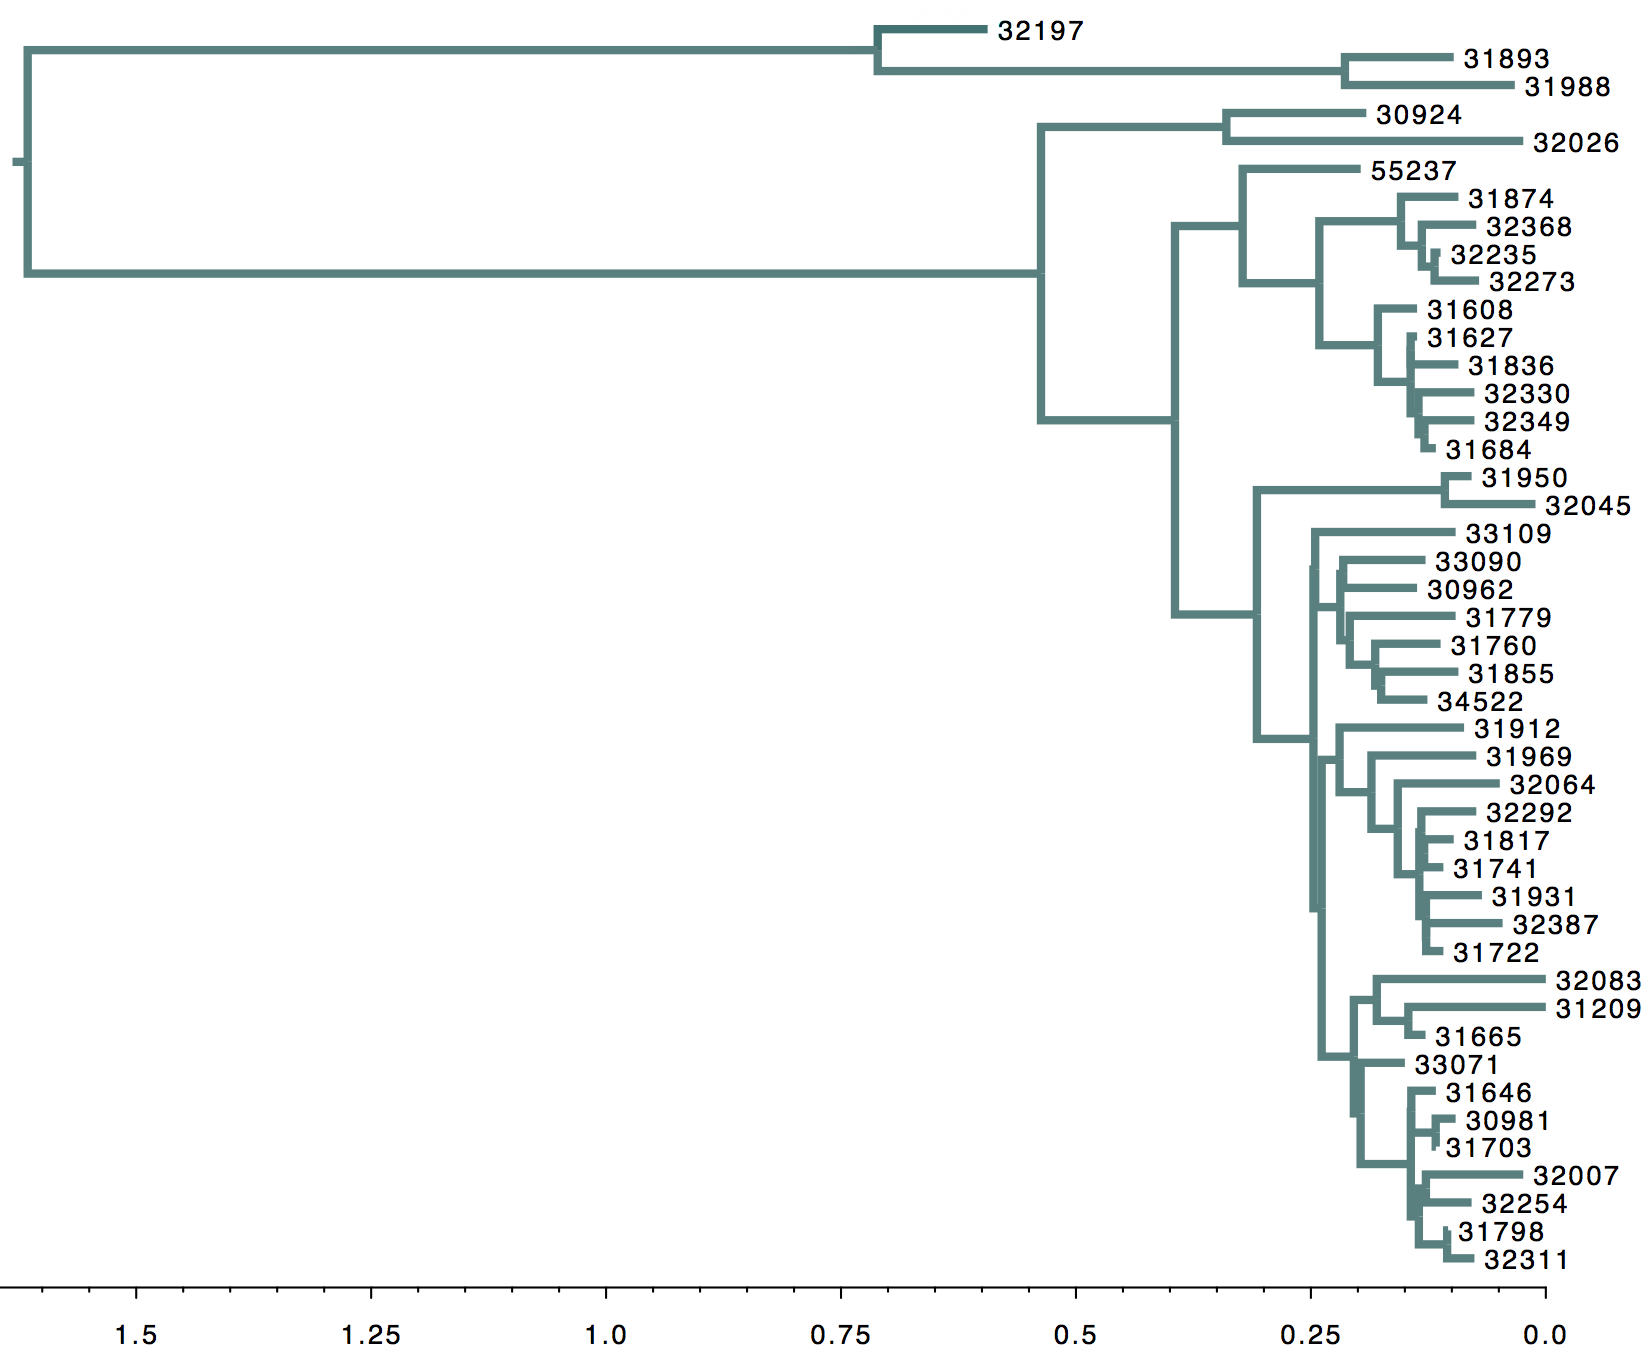
\includegraphics[width=2.25in]{H1N1_stochSIR_fluTree2.png}
}
\quad
{%
    	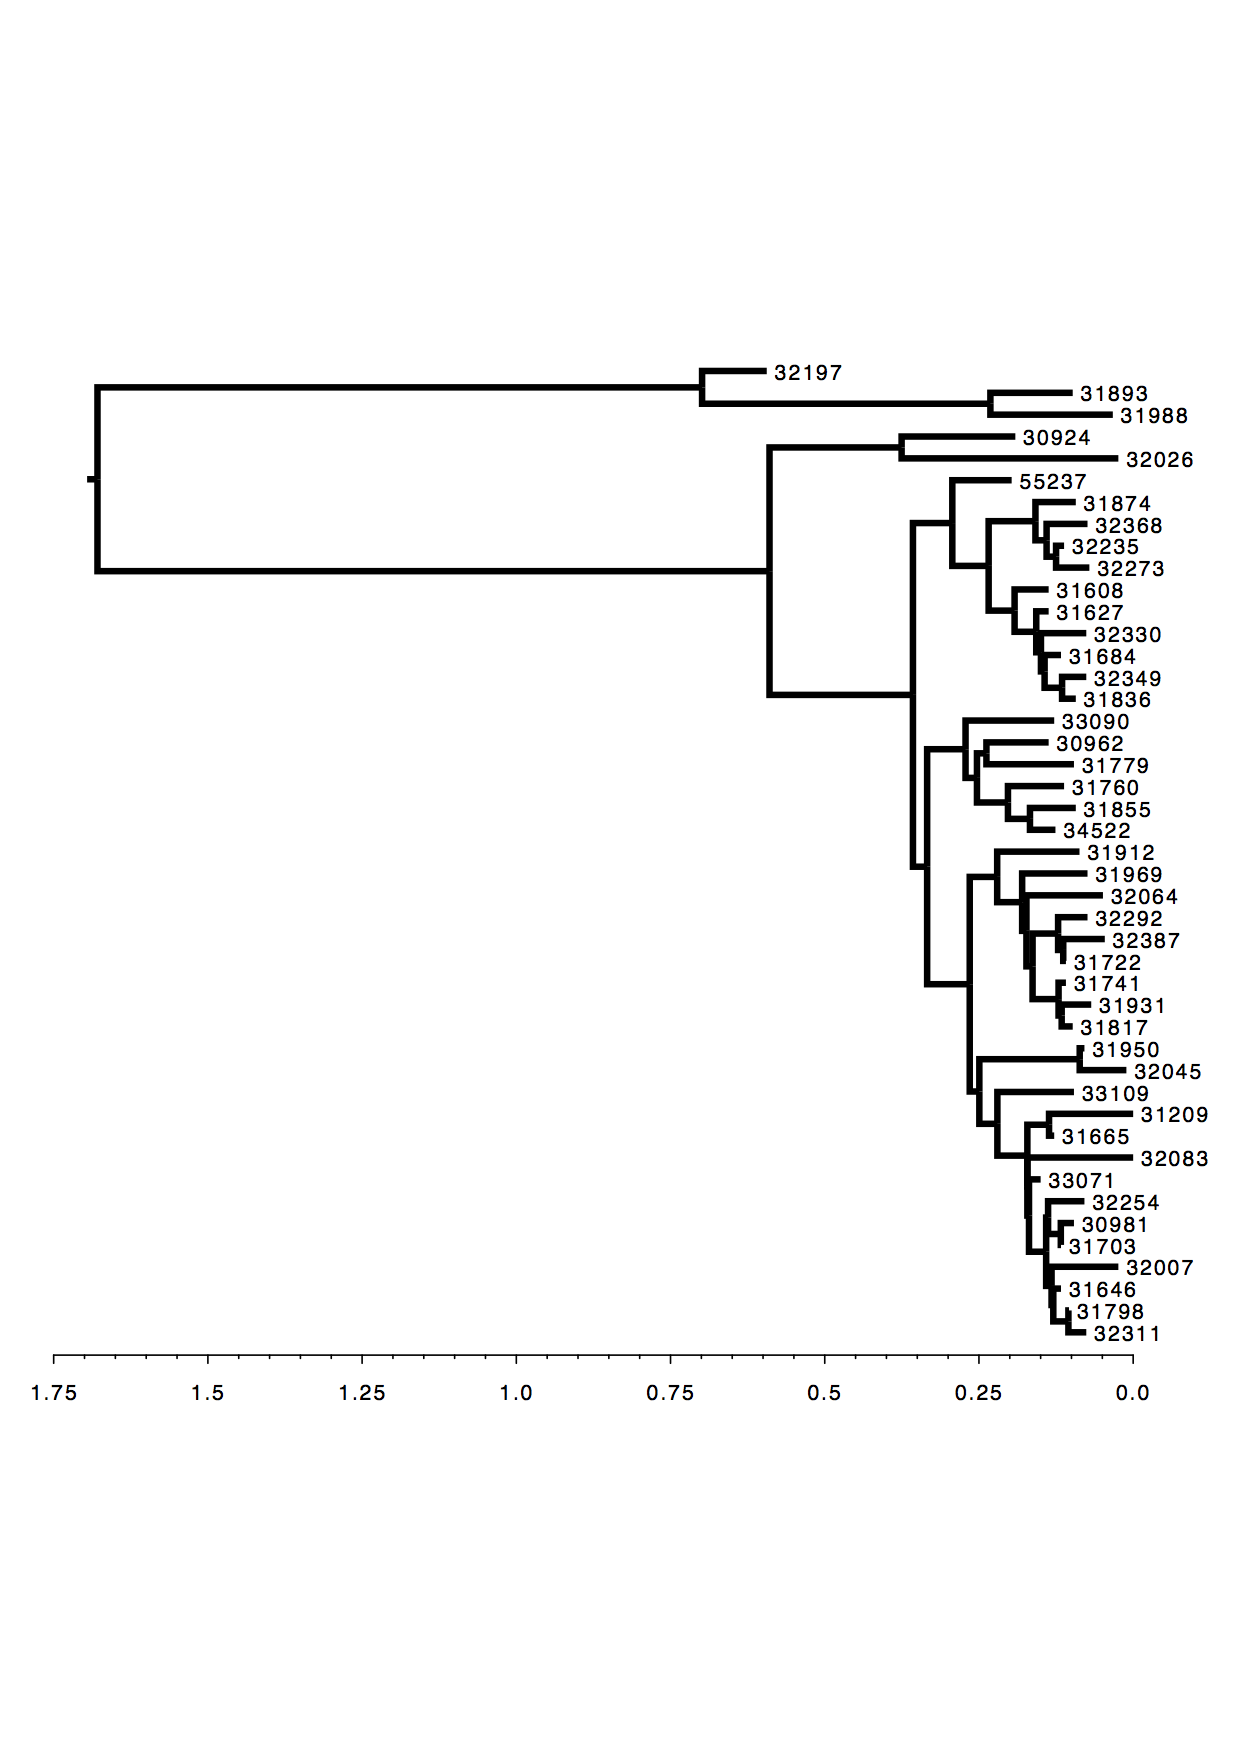
\includegraphics[width=2.25in]{H1N1_deterSIR_fluTree2.png}
}
\quad
{%
    	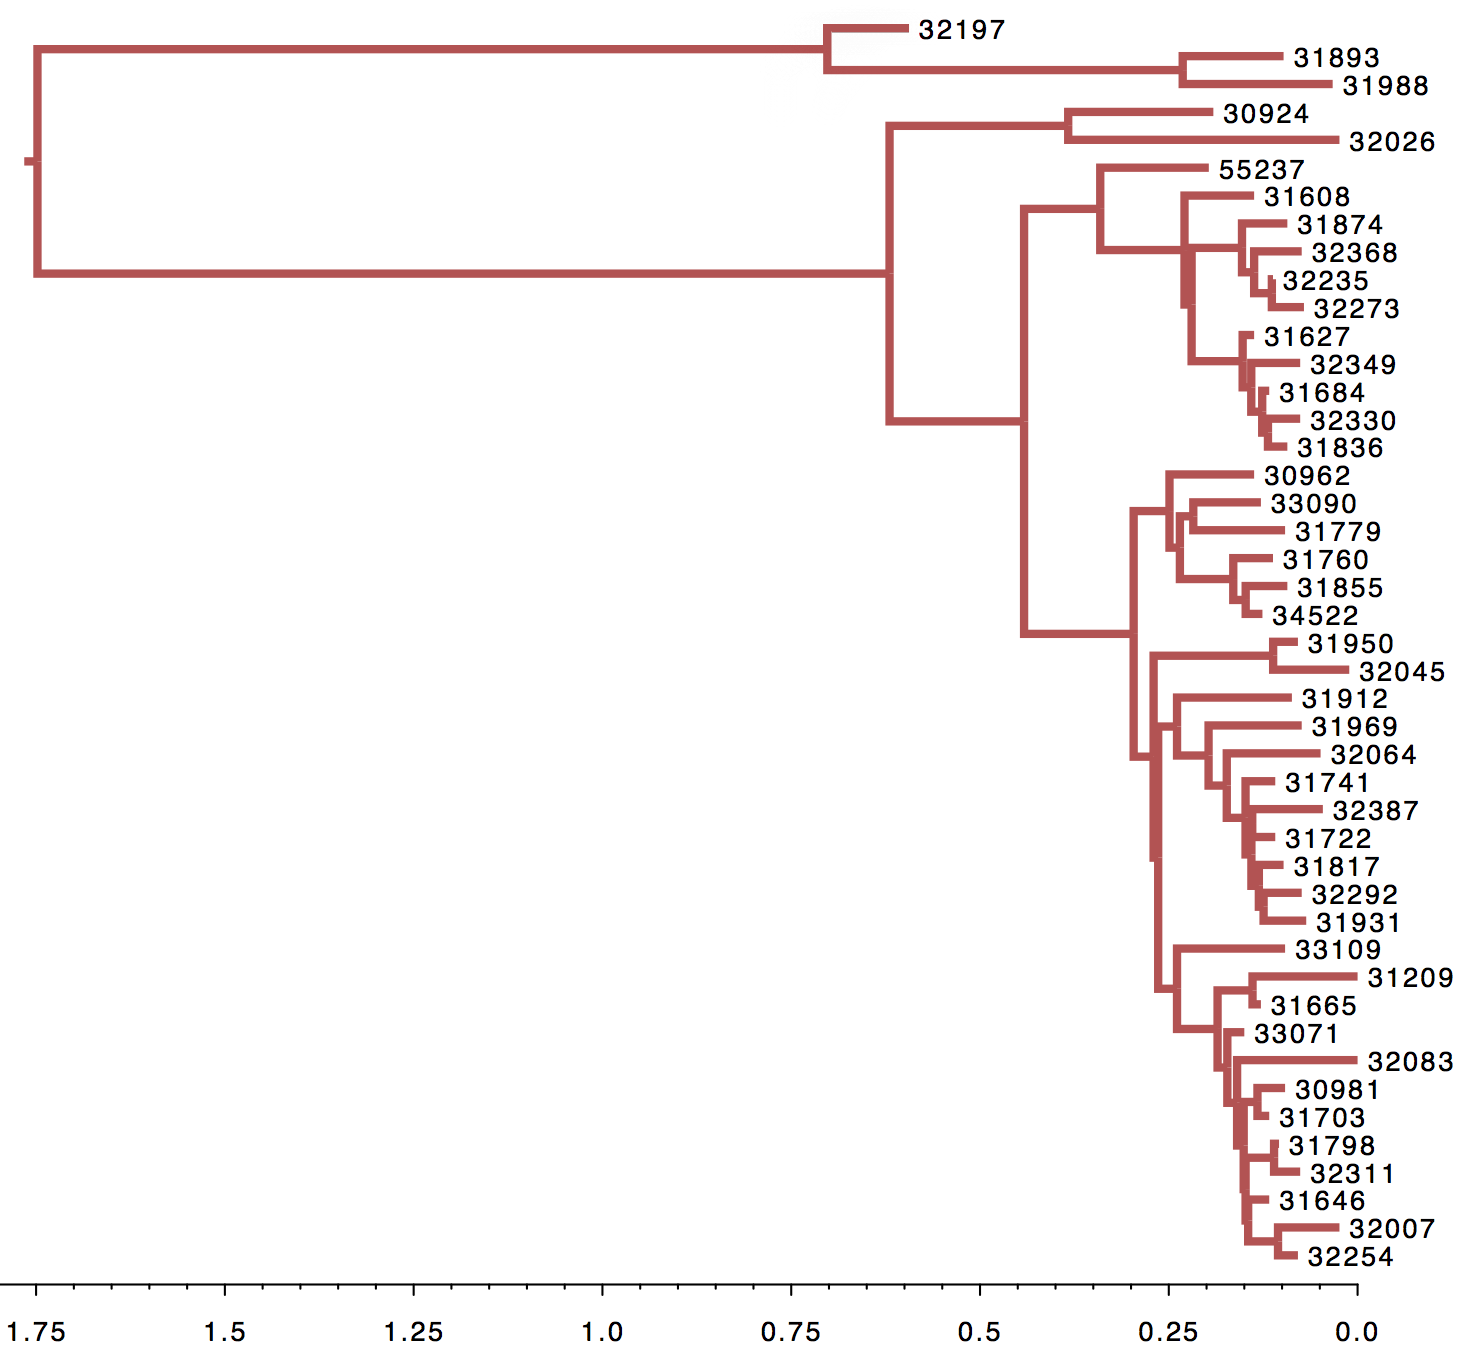
\includegraphics[width=2.25in]{H1N1_BDSIR_fluTree2.png}
}
\caption{Representative influenza A (H1N1) posterior trees from inference using the \stochCoalSIR{} (left), \deterCoalSIR{} (right), \BDSIR{} (bottom) models.
}
\end{figure}
%
%
\begin{figure}[!ht]
\begin{center}
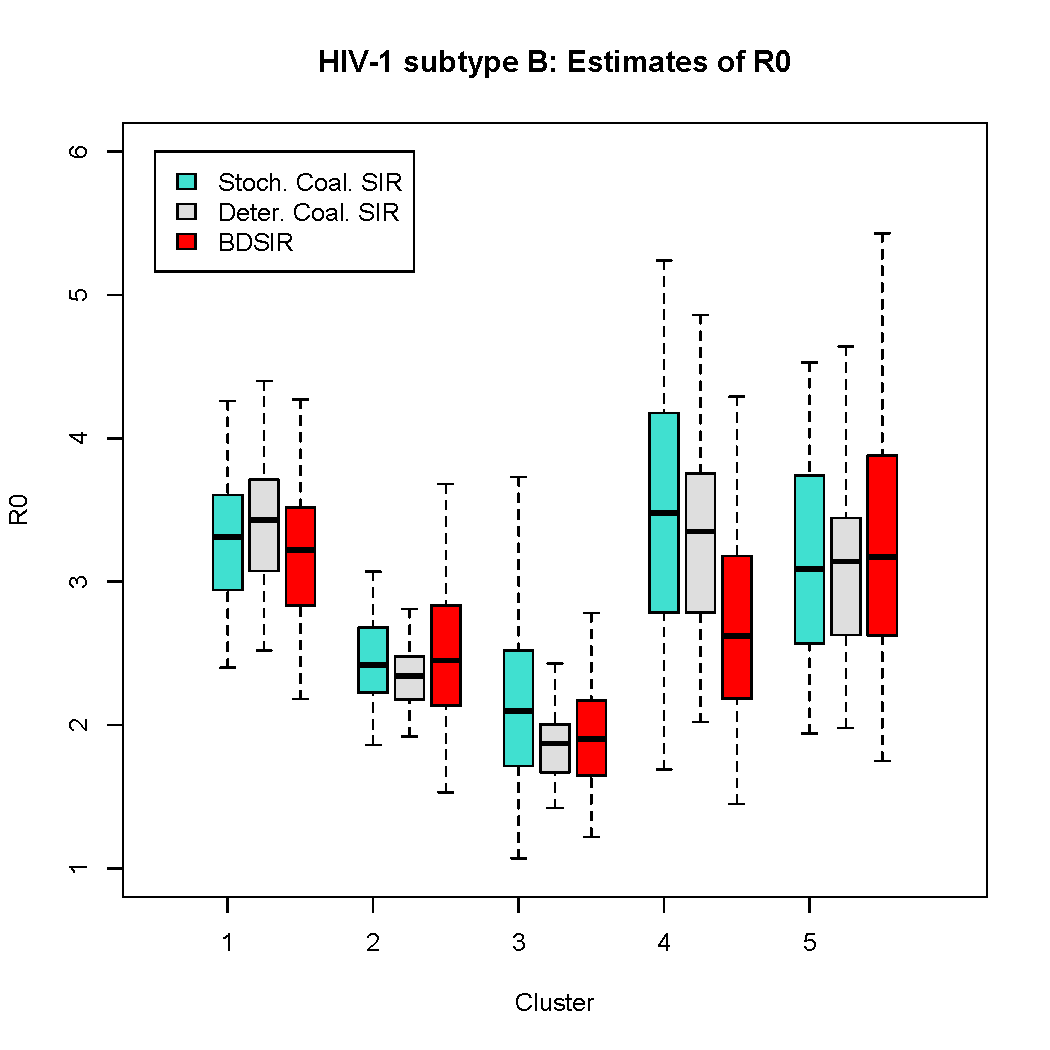
\includegraphics[width=\textwidth]{HIV1subtypeB_R0.pdf}
\end{center}
\caption{
95\% HPD intervals of $R_0$ for the HIV-1 subtype B UK cluster 
analyses using coalescent and birth-death methods.}
\label{fig:HIV_R0}
\end{figure}
%
\begin{figure}[!ht]
\begin{center}
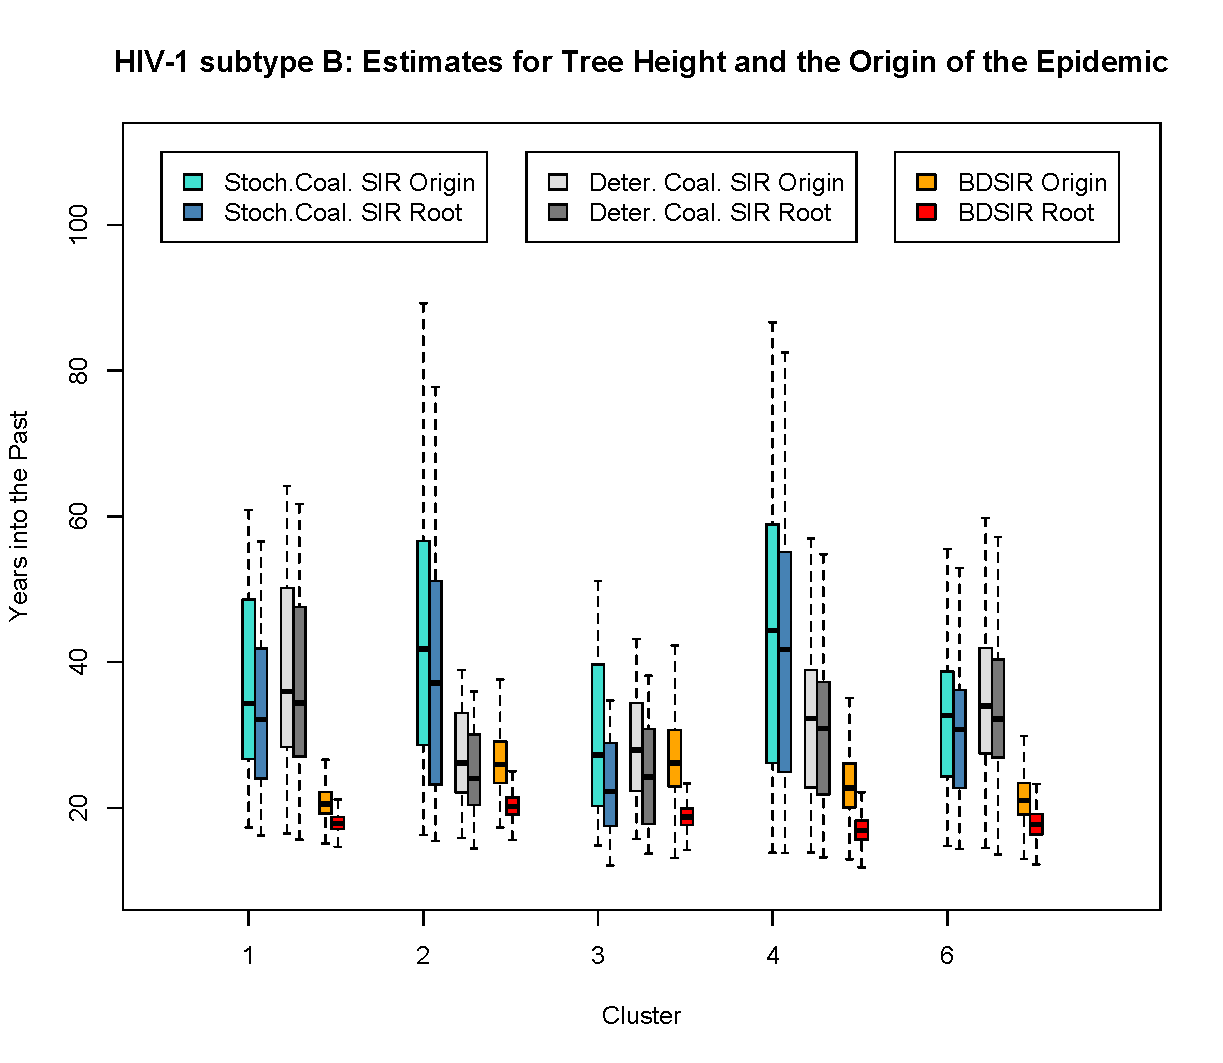
\includegraphics[width=\textwidth]{HIV1subtypeB_treeHeight_Origin.pdf}
\end{center}
\caption{
95\% HPD intervals for coalescent [\protect\cite{Volz:2012}] and birth-death [\protect\cite{Kuhnert:2014}]
estimations of the time into the past at which the root of the HIV-1 tree and introduction 
of the first infection occurred.}
\label{fig:HIV_HeightandOrigin}
\end{figure}
%
\begin{figure}[!ht]
\begin{center}
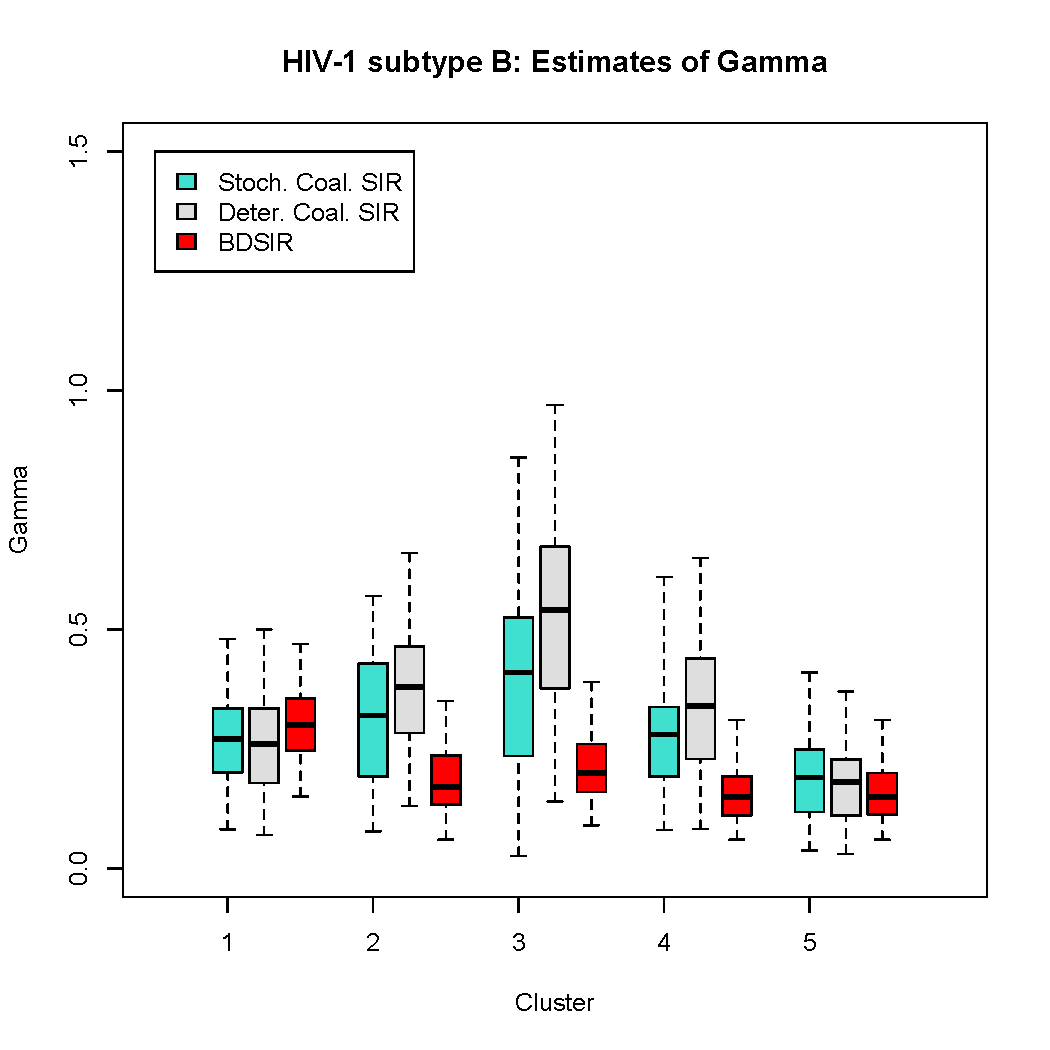
\includegraphics[width=\textwidth]{HIV1subtypeB_gamma.pdf}
\end{center}
\caption{
95\% HPD intervals of $\gamma$ for the HIV-1 subtype B UK cluster 
analyses using coalescent and birth-death methods.}
\label{fig:HIV_gamma}
\end{figure}
%
\begin{figure}[!ht]
\begin{center}
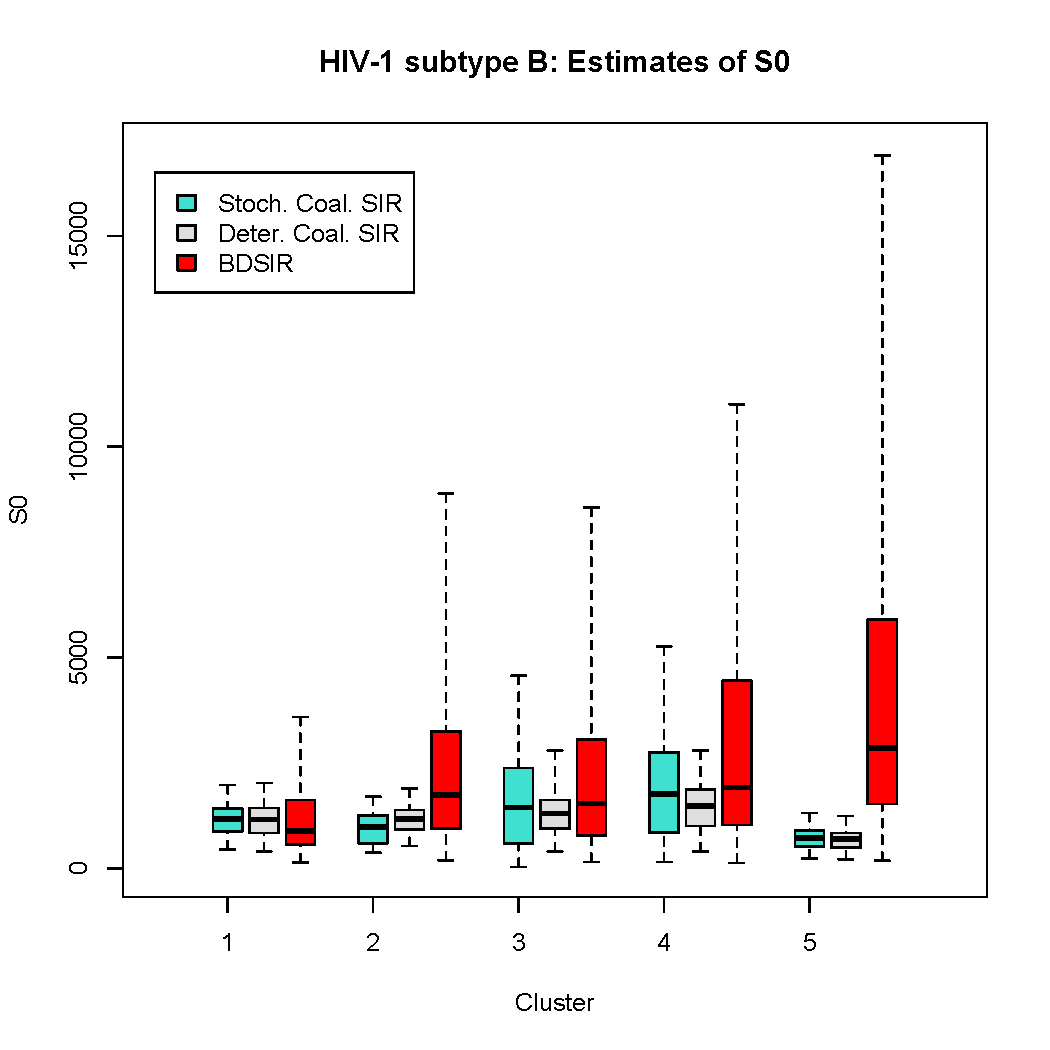
\includegraphics[width=\textwidth]{HIV1subtypeB_S0.pdf}
\end{center}
\caption{95\% HPD intervals of $S_0$ for the HIV-1 subtype B UK cluster 
analyses using coalescent and birth-death methods.}
\label{fig:HIV_S0}
\end{figure}
%
%
\begin{table}[!ht]
\begin{center}
\caption{\large{Simulation Study Results for Stochastic Coalescent Trees}}
\begin{tabular}{|c|c|c|c|c|c|c|c|c|}
\hline
$\eta$ & Inference & Truth & Mean & Median & Error & Bias & Relative & 95\% HPD \\ 
&  &  &  &  &  &  &  HPD width & accuracy \\ 
	\hline
	\hline
$\mathcal{R}_0$ & Stoch.Coal.SIR & 2.50 & 2.81 & 2.64 & 0.11 & 0.08 & 0.95 & 100.00\% \\
& Deter.Coal.SIR & 2.50 & 2.73 & 2.65 & 0.14 & 0.06 & 0.85 & 96.00\% \\
   \hline
   \hline 
$\gamma$ & Stoch.Coal.SIR & 0.30 & 0.28 & 0.26 & 0.16 & -0.11 & 1.17 & 99.00\% \\
& Deter.Coal.SIR & 0.30 & 0.30 & 0.28 & 0.18 & -0.03 & 1.20 & 99.00\% \\
   \hline
   \hline
$S_{(0)}$ & Stoch.Coal.SIR & 999 & 1456 & 986 & 0.21 & 0.02 & 3.93 & 100.00\% \\
& Deter.Coal.SIR & 999 & 1720 & 1057 & 0.48 & 0.24 & 4.28 & 99.00\% \\
   \hline
   \hline
$z_{(0)}$ & Stoch.Coal.SIR & (varies) & 42.36 & 40.43 & 0.03 & 0.02 & 0.20 & 98.00\% \\
& Deter.Coal.SIR & (varies) & 41.25 & 39.77 & 0.03 & 0.01 & 0.07 & 64.00\% \\ 
   \hline
\end{tabular}
\end{center}
\label{table:simStochCoalTrees}
 \end{table}
%
\clearpage

\begin{table}[!ht]
\begin{center}
\caption{\large{Simulation Study Results for Deterministic Coalescent Trees}}
\begin{tabular}{|c|c|c|c|c|c|c|c|c|}
\hline
$\eta$ & Inference & Truth & Mean & Median & Error & Bias & Relative & 95\% HPD \\ 
&  &  &  &  &  &  &  HPD width & accuracy \\ 
	\hline
	\hline
$\mathcal{R}_0$ & Stoch.Coal.SIR & 2.50 & 2.44 & 2.37 & 0.06 & -0.05 & 0.67 & 100.00\% \\
& Deter.Coal.SIR & 2.50 & 2.51 & 2.46 & 0.08 & -0.01 & 0.59 & 99.00\% \\
   \hline
   \hline 
$\gamma$ & Stoch.Coal.SIR & 0.30 & 0.33 & 0.31 & 0.07 & 0.05 & 1.00 & 100.00\% \\
& Deter.Coal.SIR & 0.30 & 0.32 & 0.30 & 0.10 & 0.02 & 0.79 & 100.00\% \\
   \hline
   \hline
$S_{(0)}$ & Stoch.Coal.SIR & 999 & 1586 & 1142 & 0.26 & 0.20 & 3.83 & 100.00\% \\
& Deter.Coal.SIR & 999 & 1426 & 1030 & 0.36 & 0.13 & 3.03 & 100.00\% \\
   \hline
   \hline
$z_{(0)}$ & Stoch.Coal.SIR & 44.12 & 45.52 & 44.74 & 0.02 & 0.01 & 0.19 & 93.00\% \\
& Deter.Coal.SIR & 44.12 & 44.34 & 44.11 & 0.02 & 1.93\mbox{\sc{e}-3} & 0.08 & 92.00\% \\
   \hline
\end{tabular}
\end{center}
\label{table:simDetCoalTrees}
 \end{table}
%
%
\clearpage
\begin{table}[!ht]
\begin{center}
\caption{\large{Results for Homochronous Sampling}}
\begin{tabular}{|c|c|c|c|c|c|c|c|c|}
\hline
$\eta$ & Inference & Truth & Mean & Median & Error & Bias & Relative & 95\% HPD \\ 
&  &  &  &  &  &  &  HPD width & accuracy \\ 
	\hline
	\hline
$\mathcal{R}_0$ & Stoch.Coal.SIR & 2.50 & 3.04 & 2.74 & 0.13 & 0.11 & 1.32 & 100.00\% \\
& Deter.Coal.SIR & 2.50 & 4.05 & 3.29 & 0.34 & 0.32 & 2.38 & 100.00\% \\
& BDSIR & 2.50 & 2.84 & 2.49 & 0.16 & 0.03 & 1.45 & 97.00\% \\
   \hline
   \hline 
$\gamma$ & Stoch.Coal.SIR & 0.30 & 0.26 & 0.23 & 0.25 & -0.21 & 1.43 & 100.00\% \\
& Deter.Coal.SIR & 0.30 & 0.26 & 0.19 & 0.36 & -0.31 & 2.03 & 100.00\% \\
& BDSIR & 0.30 & 0.23 & 0.17 & 0.42 & -0.42 & 2.04 & 100.00\% \\
   \hline
   \hline
$S_{(0)}$ & Stoch.Coal.SIR & 999 & 1660 & 1065 & 0.18 & 0.09 & 4.75 & 100.00\% \\
& Deter.Coal.SIR & 999 & 4127 & 679 & 0.78 & 0.09 & 10.24 & 100.00\% \\
& BDSIR & 999 & 1907 & 1320 & 0.41 & 0.41 & 4.86 & 100.00\% \\
   \hline
   \hline
$z_{(0)}$ & Stoch.Coal.SIR & 20.0 & 20.17 & 19.82 & 0.09 & -0.03 & 0.43 & 95.00\% \\
& Deter.Coal.SIR & 20.0 & 19.09 & 19.21 & 0.09 & -0.05 & 0.19 & 73.00\% \\
& BDSIR & 20.0 & 36.56 & 29.38 & 0.55 & 0.54 & 4.24 & 100.00\% \\
    \hline
\end{tabular}
\end{center}
\label{table:simDetCoalTrees}
 \end{table}
%
%
\clearpage
 \begin{table}[!ht]
\begin{center}
\caption{
\large{Simulation Study Results: The Effect of Broader Priors on Deterministic Coalescent SIR}}
\label{table:simLowerS0broadPriors}
\end{center}
\begin{tabular}{|c|c|c|c|c|c|c|c|c|}
\hline
$\eta$ & St. Dev. & Truth & Mean & Median & Error & Bias & Relative & 95\% HPD \\ 
&  &  &  &  &  &  & HPD width & accuracy \\ 
	\hline
	\hline
$\mathcal{R}_0$ & 2 & 1.50 & 2.06 & 1.75 & 0.40 & 0.35 & 0.86 & 79.00\% \\
$\mathcal{R}_0$ & 1 & 1.50 & 1.80 & 1.49 & 0.24 & 0.15 & 0.52 & 85.00\% \\
$\mathcal{R}_0$ & 2 & 2.50 & 3.31 & 2.85 & 0.34 & 0.24 & 1.43 & 95.00\% \\
$\mathcal{R}_0$ & 1 & 2.50 & 2.68 & 2.49 & 0.13 & 0.04 & 0.80 & 99.00\% \\
   \hline
   \hline 
$\gamma$ & 2 & 0.30 & 0.31 & 0.23 & 0.37 & -0.12 & 1.59 & 96.00\% \\
$\gamma$ & 1 & 0.30 & 0.26 & 0.23 & 0.27 & -0.22 & 1.15 & 89.00\% \\
$\gamma$ & 2 & 0.30 & 0.31 & 0.25 & 0.33 & -0.09 & 1.59 & 95.00\% \\
$\gamma$ & 1 & 0.30 & 0.32 & 0.29 & 0.16 & 3.14\mbox{\sc{e}-3} & 1.27 & 99.00\% \\
   \hline
   \hline
$S_{(0)}$ & 2 & 499 & 2041 & 249 & 1.40 & 0.49 & 7.75 & 85.00\% \\
$S_{(0)}$ & 1 & 499 & 562 & 361 & 0.44 & -0.26 & 3.36 & 91.00\% \\
$S_{(0)}$ & 2 & 999 & 3028 & 717 & 1.05 & 0.33 & 6.60 & 94.00\% \\
$S_{(0)}$ & 1 & 499 & 553.38 & 337 & 0.42 & -0.26 & 3.08 & 92.00\% \\
   \hline
   \hline
$z_{(0)}$ & 2 & (varies) & 65.10 & 62.01 & 0.04 & 0.03 & 0.25 & 86.00\% \\
$z_{(0)}$ & 1 & (varies) & 91.03 & 72.51 & 0.39 & 0.38 & 0.42 & 88.00\% \\
$z_{(0)}$ & 2 & (varies) & 40.97 & 39.85 & 0.03 & -6.78\mbox{\sc{e}-4} & 0.08 & 81.00\% \\
$z_{(0)}$ & 1 & (varies) & 112.79 & 90.37 & 0.26 & 0.26 & 0.94 & 85.00\% \\
   \hline
\end{tabular}
\end{table}
%
%
\begin{table}[!ht]
\begin{center}
\caption{\large{Comparison of Computation Times for Bayesian Inference of Epidemic Parameters from Genetic Sequence Data using SIR Models}}
\vspace{3mm}
\label{table:compTime}
\begin{tabular}{|c|c|c|}
\hline
Data Type & Inference Model & Mean time per million \\ 
 &  &  samples (MCMC) \\ 
	\hline
& Stoch.Coal.SIR & 20m 41s \\
Sim. Study ($R_{0} \approx 2.50$) & Deter.Coal.SIR & 3m 27s \\
& BDSIR & 56m 27s \\
   \hline 
& Stoch.Coal.SIR & 1h 43m 30s \\
Sim. Study ($R_{0} \approx 1.50$) & Deter.Coal.SIR & 3m 47s \\
& BDSIR & 41m 35s \\
   \hline
& Stoch.Coal.SIR & 1h 50m 41s \\
Sim. Study ($R_{0} \approx 1.10$) & Deter.Coal.SIR & 6m 45s \\
& BDSIR & 41m 21s \\
%   \hline
%& Stoch.Coal.SIR & 25m 10s \\
%HCV & Deter.Coal.SIR & 1m 50s \\
%& BDSIR & 42m 3s \\
   \hline
& Stoch.Coal.SIR & 1h 20m 55s \\
H1N1 & Deter.Coal.SIR & 9m 44s \\
& BDSIR & 47m 33s \\
   \hline
& Stoch.Coal.SIR & 14h 37m 45s \\
HIV-1 & Deter.Coal.SIR & 7m 56s \\
& BDSIR & 1h 38m 54s \\
   \hline
\end{tabular}
\end{center}
\end{table}
%
%
\begin{table}[!ht]
\begin{center}
\caption{\large{Deterministic Coalescent SIR Results for Simulated Sequences:  
$R_{0}=1.0987$ and $S_{0}=499$, $R_{0}=1.0989$ and $S_{0}=999$, $R_{0}=1.09945$ and $S_{0}=1999$}}
\label{table:simSeq}
\begin{tabular}{|c|c|c|c|c|c|c|c|}
\hline
$\eta$ & Truth & Mean & Median & Error & Bias & Relative & 95\% HPD \\ 
&  &  &  &  &  &  HPD width & accuracy \\ 
	\hline
	\hline
%*$\mathcal{R}_0$ & $\approx$1.10 & 2.08 & 1.58 & 0.83 & 0.84 & 0.69 & 4.00\% \\
%   \hline
%*$\gamma$ & 0.30 & 0.39 & 0.25 & 0.38 & 0.01 & 1.10 & 83.00\% \\
%   \hline
%*$S_{(0)}$ & 499 & 332 & 198 & 0.59 & -0.55 & 1.87 & 81.00\% \\
%   \hline
%*$z_{(0)}$ & (varies) & 95.81 & 69.68 & 0.46 & 0.35 & 0.21 & 25.00\% \\
%	\hline 
%	\hline
%	\hline
$\mathcal{R}_0$ & $\approx$1.10 & 1.89 & 1.28 & 0.62 & 0.63 & 0.40 & 52.00\% \\
   \hline
$\gamma$ & 0.30 & 0.57 & 0.44 & 0.59 & 0.52 & 2.14 & 95.00\% \\
   \hline
$S_{(0)}$ & 499 & 1830 & 1222 & 1.50 & 1.31 & 11.49 & 96.00\% \\
   \hline
$z_{(0)}$ & (varies) & 109.55 & 76.21 & 0.61 & 0.54 & 0.35 & 37.00\% \\
	\hline
	\hline
	\hline
$\mathcal{R}_0$ & $\approx$1.10 & 1.55 & 1.35 & 0.25 & 0.25 & 0.45 & 16.00\% \\
   \hline
$\gamma$ & 0.30 & 0.27 & 0.24 & 0.20 & -0.12 & 1.23 & 61.00\% \\
   \hline
$S_{(0)}$ & 999 & 1293 & 804 & 0.27 & -0.10 & 3.58 & 64.00\% \\
   \hline
$z_{(0)}$ & (varies) & 117.39 & 99.75 & 0.25 & 0.18 & 0.23 & 23.00\% \\
	\hline
	\hline
	\hline
$\mathcal{R}_0$ & $\approx$1.10 & 1.37 & 1.22 & 0.16 & 0.16 & 0.28 & 40.00\% \\
   \hline
$\gamma$ & 0.30 & 0.26 & 0.24 & 0.18 & -0.14 & 1.13 & 64.00\% \\
   \hline
$S_{(0)}$ & 1999 & 2292 & 1531 & 0.23 & -0.18 & 3.45 & 66.00\% \\
   \hline
$z_{(0)}$ & (varies) & 150.39 & 138.69 & 0.23 & 0.20 & 0.32 & 18.00\% \\
   \hline
\end{tabular}
\end{center}
\end{table}
%
\begin{table}[!ht]
\begin{center}
\caption{\large{Simulation Study Details}}
\vspace{3mm}
\label{table:simSeq}
\begin{tabular}{|c|c|}
\hline
\bf{Type of simulated data} & \bf{Inference models used} \\ 
	\hline
	\hline
1. Varying $R_0$ and $S_0$ (orig.) &  \\
(a) $R_{0}\approx 1.1$, $S_{0}=499$, $\gamma=0.25$, $\psi=0.15$ & Deter.Coal.SIR, Stoch.Coal.SIR, BDSIR \\
(b) $R_{0}\approx 1.2$, $S_{0}=499$, $\gamma=0.30$, $\psi=0.15$ & Deter.Coal.SIR \\
(c) $R_{0}\approx 1.5$, $S_{0}=499$, $\gamma=0.30$, $\psi=0.15$ & Deter.Coal.SIR, Stoch.Coal.SIR, BDSIR \\
(d) $R_{0}\approx 1.5$, $S_{0}=999$, $\gamma=0.30$, $\psi=0.20$ & Deter.Coal.SIR, Stoch.Coal.SIR, BDSIR \\
(e) $R_{0}\approx 2.5$, $S_{0}=999$, $\gamma=0.30$, $\psi=0.05$ & Deter.Coal.SIR, Stoch.Coal.SIR, BDSIR \\
   \hline
   \hline
2. Varying $S_0$ for fixed $R_0$ &  \\
(a) $R_{0}\approx 1.1$, $S_{0}=499$, $\gamma=0.25$, $\psi=0.15$ & Deter.Coal.SIR, Stoch.Coal.SIR, BDSIR \\
(f) $R_{0}\approx 1.1$, $S_{0}=999$, $\gamma=0.30$, $\psi=0.20$ & Deter.Coal.SIR \\
(g) $R_{0}\approx 1.1$, $S_{0}=1999$, $\gamma=0.30$, $\psi=0.09$ & Deter.Coal.SIR \\
   \hline
   \hline
3. Contemporaneous sampling & \\
(d) $R_{0}\approx 1.5$, $S_{0}=999$, $\gamma=0.30$, $\psi=0.20$ & Deter.Coal.SIR, Stoch.Coal.SIR, BDSIR \\
(e) $R_{0}\approx 2.5$, $S_{0}=999$, $\gamma=0.30$, $\psi=0.05$ & Deter.Coal.SIR, Stoch.Coal.SIR, BDSIR \\
   \hline
   \hline
4. Phylogenetic uncertainty &  \\
(e) $R_{0}\approx 2.5$, $S_{0}=999$, $\gamma=0.30$, $\psi=0.05$ & Deter.Coal.SIR, Stoch.Coal.SIR, BDSIR \\	
   \hline
   \hline
5. Reparameterization (growth rate) &  \\
(e) $R_{0}\approx 2.5$, $S_{0}=999$, $\gamma=0.30$, $\psi=0.05$ & Deter.Coal.SIR \\
   \hline
\end{tabular}
\end{center}
\end{table}
%
\begin{table}[!ht]
\footnotesize
\begin{center}
\caption{
\large{Epidemic Parameter Estimations from HIV-1 Subtype B Sequence Data}}
\vspace{5mm}
\label{table:HIV}
\begin{tabular}{|c|c|c|c|c|c|}
  \hline
\uline{Inference Model} & $R_0$ & $\gamma$ & $S_0$ & Root of & Origin $z_{0}$ of the \\ 
HIV cluster & & & & the tree (yr) & epidemic (yr) \\
   \hline
   \hline
    & & & & &\\
\bf{\StochCoalSIR} & & & & &\\
------------------ & & & & & \\
Cluster 1 & 3.31 & 0.27 & 1165 & 1971 & 1969 \\ 
 & (2.40 - 4.26) & (8.17E-2 - 0.48) & (448 - 1974) & (1946-1987) & (1942-1986) \\
Cluster 2 & 2.42 & 0.32 & 976 & 1975 & 1972 \\ 
 & (1.86 - 3.07) & (7.72E-2 - 0.57) & (371 - 1701) & (1953 - 1988) & (1947 - 1988) \\
Cluster 3 & 2.10 & 0.41 & 1442 & 1979 & 1973 \\ 
 & (1.07 - 3.73) & (2.59\mbox{\sc{e}-2} - 0.86) & (33 - 4568) & (1959 - 1990) & (1943 - 1989) \\
Cluster 4 & 3.48 & 0.28 & 1757 & 1964 & 1961 \\ 
 & (1.69 - 5.24) & (0.08 - 0.61) & (148 - 5260) & (1922 - 1990) & (1918 - 1991) \\
Cluster 6 & 3.09 & 0.19 & 727 & 1972 & 1970 \\ 
 & (1.94 - 4.53) & (3.72\mbox{\sc{e}-2} - 0.41) & (236 - 1312) & (1950 - 1989) & (1947 - 1988) \\
   \hline
   \hline
   & & & & &\\
\bf{\DeterCoalSIR} & & & & &\\
-------------------- & & & & & \\
Cluster 1 & 3.43 & 0.26 & 1158 & 1969 & 1967 \\ 
 & (2.52 - 4.40) & (6.95E-2 - 0.50) & (397 - 2023) & (1941-1987) & (1939-1986) \\
Cluster 2 & 2.34 & 0.38 & 1163 & 1979 & 1977 \\ 
 & (1.92 - 2.81) & (0.13 - 0.66) & (530 - 1895) & (1967 - 1989) & (1964 - 1987) \\
Cluster 3 & 1.87 & 0.54 & 1298 & 1979 & 1975 \\ 
 & (1.42 - 2.43) & (0.14 - 0.97) & (399 - 2267) & (1965 - 1989) & (1960 - 1987) \\
Cluster 4 & 3.35 & 0.34 & 1479 & 1972 & 1971 \\ 
 & (2.02 - 4.86) & (8.22\mbox{\sc{e}-2} - 0.65) & (397 - 2792) & (1948 - 1990) & (1946 - 1989) \\
Cluster 6 & 3.14 & 0.18 & 693 & 1971 & 1969 \\ 
 & (1.98 - 4.64) & (2.99\mbox{\sc{e}-2} - 0.37) & (213 - 1241) & (1949 - 1989) & (1943 - 1988) \\
   \hline
   \hline
   & & & & &\\
\bf{\BDSIR{}} & & & & &\\ 
--------------- & & & & & \\
Cluster 1 & 3.22 & 0.30 & 880 & 1986 & 1983 \\ 
 & (2.18-4.27) & (0.15-0.47) & (142-3592) & (1983-1988) & (1978-1987) \\
Cluster 2 & 2.45 & 0.17 & 1745 & 1983 & 1978 \\ 
& (1.53-3.68) & (0.06-0.35) & (190-8892) & (1979-1986) & (1968-1984) \\ 
Cluster 3 & 1.90 & 0.20 & 1540 & 1985 & 1978 \\ 
 & (1.22-2.78) & (0.09-0.39) & (153-8558) & (1981-1988) & (1962-1986) \\ 
Cluster 4 & 2.62 & 0.15 & 1921 & 1987 & 1981 \\ 
 & (1.45-4.29) & (0.06-0.31) & (128-11007) & (1983-1990) & (1970-1988) \\ 
Cluster 6 & 3.17 & 0.15 & 2862 & 1986 & 1983 \\  
 & (1.73-5.43) & (0.06-0.31) & (183-16909) & (1981-1989) & (1975-1989) \\ 
   \hline
\end{tabular}
\end{center}
\end{table}
%
%
\begin{table}[!ht]
\small
\begin{center}
\caption{
\large{Deterministic Coalescent SIR Results from Trees Simulated with Higher $S_0$ (with Fixed $R_0$) 
and Higher $R_{0}$ (with Fixed $S_0$)}}
\vspace{3mm}
\begin{tabular}{|c|c|c|c|c|c|c|c|}
\hline
$\eta$ & Truth & Mean & Median & Error & Bias & Relative & 95\% HPD \\ 
&  &  &  &  &  &  HPD width & accuracy \\ 
	\hline
	\hline
$\mathcal{R}_0$ & 2.50 & 2.68 & 2.49 & 0.13 & 0.04 & 0.81 & 98.00\% \\
   \hline 
$\gamma$ & 0.30 & 0.32 & 0.29 & 0.16 & 3.14\mbox{\sc{e}-3} & 1.27 & 99.00\% \\
   \hline
$S_{(0)}$ & 999 & 1807 & 1133 & 0.52 & 0.29 & 4.59 & 98.00\% \\
   \hline
$z_{(0)}$ & (varies) & 41.17 & 39.99 & 0.03 & 0.01 & 0.07 & 76.00\% \\
	\hline
	\hline
$\mathcal{R}_0$ & 2.50 & 3.28 & 2.97 & 0.23 & 0.20 & 1.42 & 100.00\% \\
   \hline
$\gamma$ & 0.35 & 0.30 & 0.28 & 0.24 & -0.20 & 1.28 & 99.00\% \\
   \hline
$S_{(0)}$ & 4999 & 7733 & 4838 & 0.34 & 0.03 & 4.18 & 100.00\% \\
   \hline
$z_{(0)}$ & (varies) & 37.45 & 36.15 & 0.03 & 1.48e-3 & 0.06 & 56.00\% \\
	\hline
	\hline
$\mathcal{R}_0$ & 2.50 & 3.76 & 3.05 & 0.26 & 0.23 & 1.50 & 100.00\% \\
   \hline
$\gamma$ & 0.40 & 0.33 & 0.31 & 0.26 & -0.22 & 1.22 & 100.00\% \\
   \hline
$S_{(0)}$ & 9999 & 12,609 & 7405 & 0.35 & -0.15 & 3.31 & 100.00\% \\
   \hline
$z_{(0)}$ & (varies) & 34.99 & 34.28 & 0.04 & -1.94e-3 & 0.05 & 43.00\% \\
	\hline
	\hline
	\hline
$\eta$ & Truth & Mean & Median & Error & Bias & Relative & 95\% HPD \\ 
&  &  &  &  &  &  HPD width & accuracy \\ 
	\hline
	\hline
$\mathcal{R}_0$ & 2.50 & 2.68 & 2.49 & 0.13 & 0.04 & 0.81 & 98.00\% \\
   \hline 
$\gamma$ & 0.30 & 0.32 & 0.29 & 0.16 & 3.14\mbox{\sc{e}-3} & 1.27 & 99.00\% \\
   \hline
$S_{(0)}$ & 999 & 1807 & 1133 & 0.52 & 0.29 & 4.59 & 98.00\% \\
   \hline
$z_{(0)}$ & (varies) & 41.17 & 39.99 & 0.03 & 0.01 & 0.07 & 76.00\% \\
	\hline
	\hline
$\mathcal{R}_0$ & 3.50 & 3.92 & 3.76 & 0.18 & 0.06 & 0.95 & 95.00\% \\
   \hline
$\gamma$ & 0.30 & 0.31 & 0.29 & 0.21 & -0.01 & 1.16 & 99.00\% \\
   \hline
$S_{(0)}$ & 999 & 1909 & 1060 & 0.64 & 0.36 & 4.26 & 100.00\% \\
   \hline
$z_{(0)}$ & (varies) & 30.65 & 30.35 & 0.04 & -6.35\mbox{\sc{e}-3} & 0.05 & 45.00\% \\
	\hline
	\hline
$\mathcal{R}_0$ & 5.00 & 6.13 & 5.53 & 0.20 & 0.12 & 1.39 & 100.00\% \\
   \hline
$\gamma$ & 0.30 & 0.28 & 0.27 & 0.29 & -0.09 & 1.18 & 100.00\% \\
   \hline
$S_{(0)}$ & 999 & 2144 & 1220 & 0.68 & 0.49 & 4.94 & 99.00\% \\
   \hline
$z_{(0)}$ & (varies) & 26.28 & 25.26 & 0.03 & -0.01 & 0.03 & 52.00\% \\
	\hline
	\hline
	\hline
$\eta$ & Truth & Mean & Median & Error & Bias & Relative & 95\% HPD \\ 
&  &  &  &  &  &  HPD width & accuracy \\ 
	\hline
	\hline
$\mathcal{R}_0$ & 5.00 & 7.20 & 6.37 & 0.27 & 0.23 & 2.53 & 100.00\% \\
   \hline
$\gamma$ & 0.30 & 0.26 & 0.22 & 0.26 & -0.19 & 1.41 & 100.00\% \\
   \hline
$S_{(0)}$ & 9999 & 17,339 & 10,518 & 0.31 & 0.12 & 4.91 & 100.00\% \\
   \hline
$z_{(0)}$ & (varies) & 28.20 & 26.93 & 0.03 & -0.01 & 1.05 & 36.00\% \\
	\hline
\end{tabular}
\end{center}
{}
\label{table:sim}
\end{table}
%
% Flush all outstanding floats
\clearpage

\bibliography{../volzSIR}
\bibliographystyle{../genetics}
\end{document}